% HaPOD tree figure for the data-driven-I lecture notebook.
%
% Adapted from the ADMOS 2023 talk (Haasdonk/Kleikamp/Ohlberger/Schindler/Wenzel),
% recolored from the WWU blue to pymor_blue.
%
% Build with:
%   latexmk -pdf hapod_tree.tex
%   pdftoppm -png -r 1200 hapod_tree.pdf hapod_tree   % -> hapod_tree-1.png, rename
%   dvisvgm --pdf hapod_tree.pdf -o hapod_tree.svg
% 1200 dpi matches the other figures in this directory.

\documentclass[11pt,border=2mm]{standalone}

\usepackage{amsmath}
\usepackage{tikz}
\usetikzlibrary{shapes.geometric,arrows,positioning,calc}

\definecolor{pymor_blue}{HTML}{3155a0}

\tikzset{treenode/.style={rectangle, text centered, draw=pymor_blue, fill=pymor_blue!30}}
\tikzset{arrow/.style={thick, ->, >=stealth}}

\begin{document}
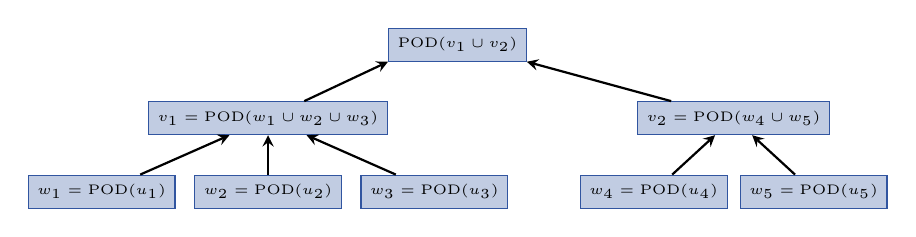
\begin{tikzpicture}[node distance=0.5cm and 0cm]
  \node[treenode] (root) {\tiny$\operatorname{POD}(v_1\cup v_2)$};

  \node[treenode, below left=of root] (child-1-1) {\tiny$v_1=\operatorname{POD}(w_1\cup w_2\cup w_3)$};
  \node[treenode, below right=of root, xshift=1.4cm] (child-1-2) {\tiny$v_2=\operatorname{POD}(w_4\cup w_5)$};

  \node[treenode, below left=of child-1-1, xshift=.35cm] (child-2-1) {\tiny$w_1=\operatorname{POD}(u_1)$};
  \node[treenode, below=of child-1-1] (child-2-2) {\tiny$w_2=\operatorname{POD}(u_2)$};
  \node[treenode, below right=of child-1-1, xshift=-.35cm] (child-2-3) {\tiny$w_3=\operatorname{POD}(u_3)$};
  \node[treenode, below left=of child-1-2, xshift=1.15cm] (child-2-4) {\tiny$w_4=\operatorname{POD}(u_4)$};
  \node[treenode, below right=of child-1-2, xshift=-1.15cm] (child-2-5) {\tiny$w_5=\operatorname{POD}(u_5)$};

  \draw[arrow] (child-1-1) -- (root.south west);
  \draw[arrow] (child-1-2) -- (root.south east);

  \draw[arrow] (child-2-1) -- (child-1-1);
  \draw[arrow] (child-2-2) -- (child-1-1);
  \draw[arrow] (child-2-3) -- (child-1-1);
  \draw[arrow] (child-2-4) -- (child-1-2);
  \draw[arrow] (child-2-5) -- (child-1-2);
\end{tikzpicture}
\end{document}
